% !TEX root = raport.tex
\documentclass{article}
\usepackage{polski}

\usepackage{amssymb}
\usepackage{amsmath}
\usepackage{mathtools}
\usepackage{graphicx}
\usepackage[includehead, left = 2cm, right = 2cm, top = 0.5cm, bottom = 2.45cm, includefoot, headheight = 10mm, footskip = 5mm]{geometry}

\setlength{\parindent}{0pt}

\begin{document}
  Podzieliłem dane na zbiory treningowy, walidacyjny, testowy w proporcjach 0.6 : 0.2 : 0.2
  Stworzyłem model regresji liniowej używający metody gradientowej dla funkcji straty MSE. Osiągnął on następujące wyniki:

  MSE

  train $\approx 14966.83$

  validation $\approx 7296.47$

  test $\approx 5250.29$

  Potem wykonałem analizę danych i zauważyłem, że najbardziej skorelowane cechy to kolejno cecha $3$, $4$ i $0$.

  % 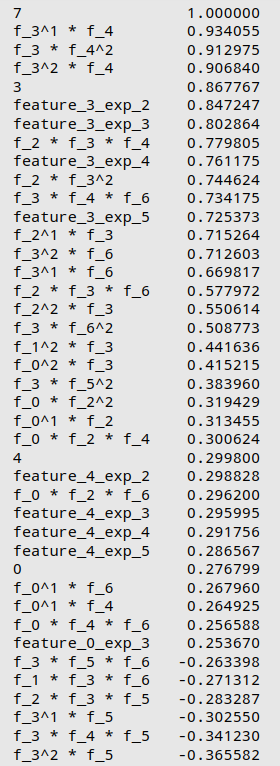
\includegraphics[width=0.8\textwidth]{Correlations.png}
  \begin{figure}
    \centering
    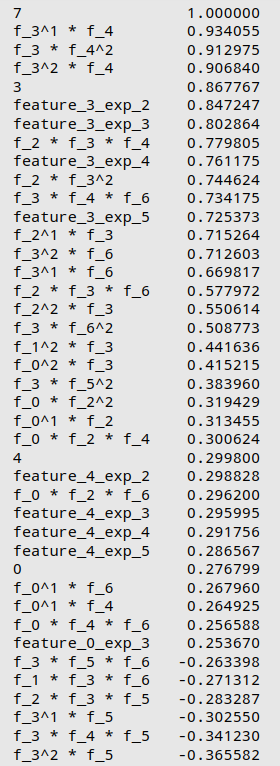
\includegraphics[width=0.2\textwidth]{Correlations.png}
    \caption{Korelacje o wartości bezwzględnej większej od $0.25$}
  \end{figure}

  Eksperymentując chciałem stworzyć model, który przewiduje wartość ostatniej cechy tylko na podstawie 
  \begin{enumerate}
    \item cechy $3$: dał validation $= 19247.740842831452$
    \item cech $3$ i $4$ dał validation $= 12340.639278231203$ 
    \item cech $0, 3, 4, [\text{cecha } 3] * [\text{cecha } 4]$ dał validation $= 5119.956974317123$
    \item cech $0, 3, 4 $  dał validation $= 7344.3616800552645$
  \end{enumerate}
  Uzyskiwały one słabe wyniki bo pomyliłem się w indeksowaniu (brałem kolumny o indeksach $3$ i $4$ z macierzy planowania a tam jest przecież dodana kolumna z jedynkami na początku) 
  oraz zapomniałem uwzględnić kolumny z jedynkami.
  Po naprawieniu tego błędu $2$ ostatnie z tych modeli uzyskały lepszy wynik na zbiorze walidacyjnym od modelu ze wszystkimi cechami.
  Najlepszy był model nr. $3$ osiągając

  MSE

  train $\approx 8314.15$
  
  validation $\approx 5119.96$
  
  test $\approx 3676.18$

  Próbowałem usuwać cechy z modelu $3$, żeby zobaczyć jak zmieni się wynik na zbiorze walidacyjnym. 
  Po usunięciu cechy $3$ wynik na zbiorze walidacyjnym zmienił się z $5119.959446855926$ na $62064.0985378222$. 

 \subsection{Początek błędu myślowego}

  Ciekawe jest, 
  że po usunięciu jeszcze cechy $4$ (czyli mamy $(0, [3]*[4])$) wynik na walidacyjnym pogorszył się tylko o około $3000$.

  Model tylko z cechą $([3*4])$ osiągnął $71178.99881227095$ na walidacyjnym. Jest to ciekawe dlatego, że wartości tej sztucznej cechy są nawet bardziej skorelowane niż wartości cechy $3$.

  Najlepszy model po dodaniu regularyzacji $L1$ pogorszył wynik na zbiorze walidacyjnym o około $100$ a na testowym polepszył o około $50$.

  Teraz próbowałem dodawać parametry do najlepszego modelu. 
  Dodawanie parametrów $1, 2,5,6$ zmieniało błąd na walidacyjnym o około $20$ (dodawałem je po jednym na raz). 
  Dodanie parametru $3$ drugi raz oraz dodanie $[3]+[4]$ nic nie zmieniło, co było spodziewane dlatego, że są one liniowo zależne od już istniejących parametrów.
  Dodanie parametrów $[0]*[3], [0]*[4]$ nie zmieniło wyniku w istotny sposób.
  Dodanie parametru $[3]^2$ polepszyło wynik na walidacyjnym o około $300$ oraz przyspieszyło zbieżność na początkowych kilku epokach. 
  Dodanie $[3]^3$ jeszcze bardziej przyspieszyło zbieżność ale pogorszyło wynik na walidacyjnym o około $500$. 

  Dodałem wszystkie parametry z $[3]^2, [3]^3, [3]^4, [3]^5, [3]^6$ co dało mi najlepszy dotąd wynik na walidacyjnym równy $4798.351894614459$. MSE pomiędzy pierwszą a drugą iteracją zmniejsza się wtedy o ponad $2\cdot 10^6$.
  Dodawanie cech w postaci $[0]^n, [4]^n$ nie poprawiało wyniku w istotny sposób.
  \subsection{Odkrycie błędu myślowego}
  Zorientowałem się, że cechy w postaci $[i]^n, [i]*[j]$ powinienem dodawać przed standaryzacją.

  \subsection{Korekta}
  Korekta pogorszyła wynik najlepszego modelu o około $2000$ na zbiorze treningowym i około $200$ na walidacyjnym.

  Dodając cechy w postaci $[3]^i$ dla $i\in\{2,\ldots, 200\}$ uzyskałem wynik na walidacyjnym równy $4368.615954268543$. 
  Dodanie $[0]^n$ oraz $[4]^n$ nie poprawiło wyniku.
  Takie obserwacje mogą sugerować, że etykiety są zależne w sposób wykładniczy od cechy $[3]$.

  Usunąłem potęgi i dodałem cechy $\exp\left(\frac{[3]-\overline{[3]}}{s}\right)$ dla $s\in\{2,\ldots,10\}$ i otrzymałem błąd
  $5037.689339105426$ na zbiorze walidacyjnym.

  Eksperymentując dalej dodałem cechę $([3]*[4])^2$ co przyniosło poprawę błędu na walidacyjnym o około $1000$. 
  Dodawanie cech $([3]*[4])^i$ dla $i > 2$ nie dawało istotniej poprawy.

  Zauważyłem swój błąd i zamieniłem cechy $\exp\left(\frac{[3]-\overline{[3]}}{s}\right)$ na $\exp\left(-\frac{\left([3]-\overline{[3]}]\right)^2}{s^2}\right)$ dla $s\in\{1, 100\}$ 
  co dało poprawę do $3099.461563941936$. Co więcej mogłem teraz usunąć cechy w postaci $[3]^n$ i dostać błąd $2774.78578867818$.

  Zastosowanie gaussowskiej funkcji bazowej dla cechy $[3]*[4]$ nie przyniosło istotnej poprawy, podobne efekty funkcja gaussowska dała dla cech $0, 4$. 
  Regularyzacja $L1$ pogorszyła wynik a $L2$ zepsuła go kompletnie (błąd $>10^6$).

  \subsection{Pewien problem z MSE}
  Zauważyłem, że moje MSE od początku miało bład w implementacji co prowadziło do błędnych wyników. 
  Co prawda nie jest to zbyt szkodliwy błąd bo rózniło się o stały czynnik od faktycznego ale unieważnia niestety moje poprzednie wyniki pod względem liczbowym. 
  Nie powinno mieć to chyba wpływu na jakość hipotez.

\end{document}
